% Use only LaTeX2e, calling the article.cls class and 12-point type.

\documentclass[12pt, notitlepage, letterpaper]{article}
\usepackage{bm,url,graphicx, amsfonts, amssymb} %PJM added these here
\usepackage{amsmath}    % need for subequations
\usepackage{graphicx}   % need for figures
\usepackage{subfigure}  % use for side-by-side figures


% The following parameters seem to provide a reasonable page setup.

% Include your paper's title here

\title{MA731: HW7}

\author{Thomas Richardson}
{\large }

% Include the date command, but leave its argument blank.

% \date{\small}



%%%%%%%%%%%%%%%%% END OF PREAMBLE %%%%%%%%%%%%%%%%



\begin{document}

% Double-space the manuscript.

\baselineskip 24pt

% Make the title.

\maketitle

\noindent

\paragraph{}

Our system is as follows:

%Equations for system, preliminaries
\begin{equation}
\label{eq:sys01}
\dot{x} = Ax + Bu
\end{equation}

\begin{equation}
\label{eq:cost}
J(x(t)) = \frac{1}{2}x(T)^TS(T)x(T) +  \frac{1}{2}\int_{0}^{T}x^TQx + u^TRu dt
\end{equation}

with
\nonumber
\begin{align}
\label{eq:ABSQRBC}
\text{A} 
&=
\begin{pmatrix}
1 & 2 \\
3 & 4
\end{pmatrix}
,&
\hfill \text{B}
&=
\begin{pmatrix}
1 \\
1
\end{pmatrix}
,&
\text{S(T)}
&=
\begin{pmatrix}
10 &  1 \\
1  & 20
\end{pmatrix}
,
\end{align}

\nonumber
\begin{align}
\text{Q} 
&=
\begin{pmatrix}
3 & 1 \\
1 & 2
\end{pmatrix}
,&
\hfill \text{R}
&=
2
,&
\hfill \text{x(0)}
&=
\begin{pmatrix}
1 \\
-1
\end{pmatrix}.
\end{align}

We first found $S(\infty)$, as a means to obtaining $K(\infty)$, which is the solution to the algebraic Riccati equation constructed from the above system:

\begin{equation}
\label{eq: ric}
-\dot{S} = A^TS + SA + Q - SBR^{-1}B^TS
\end{equation}

In the case of the ARE, we would set $\dot{S}$ equal to zero and solve to obtain $S(\infty)$.  For the given system, however, we instead simulated $S$ backwards in time as a boundary value problem, given $S(T)$, on some sufficiently large time interval, $[0, T]$, where $T$ was chosen such that the value of $S(t)$ reached some positive, symmetric, constant matrix.  This resulting matrix approximates $S(\infty)$ for our system.  In doing so, with $T = 20$, we obtained the following:

\begin{align}
\label{eq: SKinf}
S(\infty) 
&=
\begin{pmatrix}
4.37 & 4.28 \\
4.28 & 9.53
\end{pmatrix}
,&
K(\infty)
&=
\begin{pmatrix}
4.32 & 6.91 
\end{pmatrix}
\end{align}

For two different $T$ values, $T_1 = 1$ and $T_2 = 10$, we found the optimal, time dependent feedback, $K(t)$, the trajectory resulting from driving the system in Eq. \ref{eq:sys01} with the optimal feedback, and the cost, as defined above, associated with the system.  We compared these trajectories and costs to those obtained from driving the system using $K(\infty)$.  The comparison plots for each of these cases are shown below.  The costs for $T_1$ were 6.87362 ($K(\infty)$ cost) and 5.31856, and the costs for $T_2$ were 2.71506 ($K(\infty)$ cost) and 2.71496.  Note that the optimal cost for $T_1$ was found to be significantly smaller than the suboptimal cost, relative to the difference in costs for $T_2$.  Given the comparison plots for controls and trajectories, this was to be expected, as these plots for $T_2$ show that the optimal and suboptimal systems are almost indistinguishable for the system trajectories, and nearly indistinguishable for the controls until around $t = 8$, while the plots for $T_1$ show drastically different behaviors in comparison.  Therefore, for long durations, long being relative to the settling time for $S(\infty)$, we can expect similar overall behavior from the suboptimal, constant control and the optimal, time-varying control.  The implementation of a constant, stable control in practice would seem to be much easier than using a time-varying control if the outcomes from both were similar enough for the task.

\begin{figure}[h]
\begin{center}
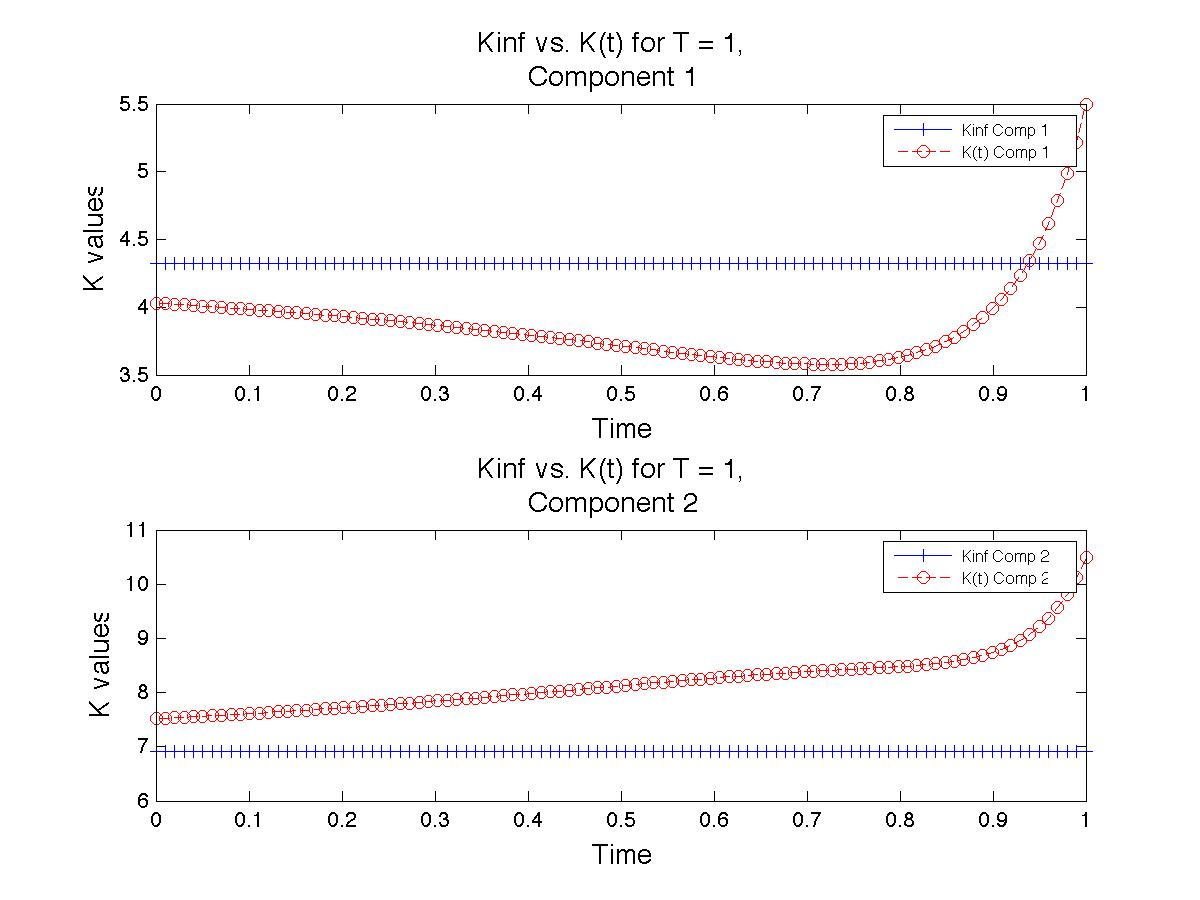
\includegraphics[width=4in]{KCompareT01}
\caption{Comparison of K's for $T_1$ }
\end{center}
\end{figure}

\begin{figure}[h]
\begin{center}
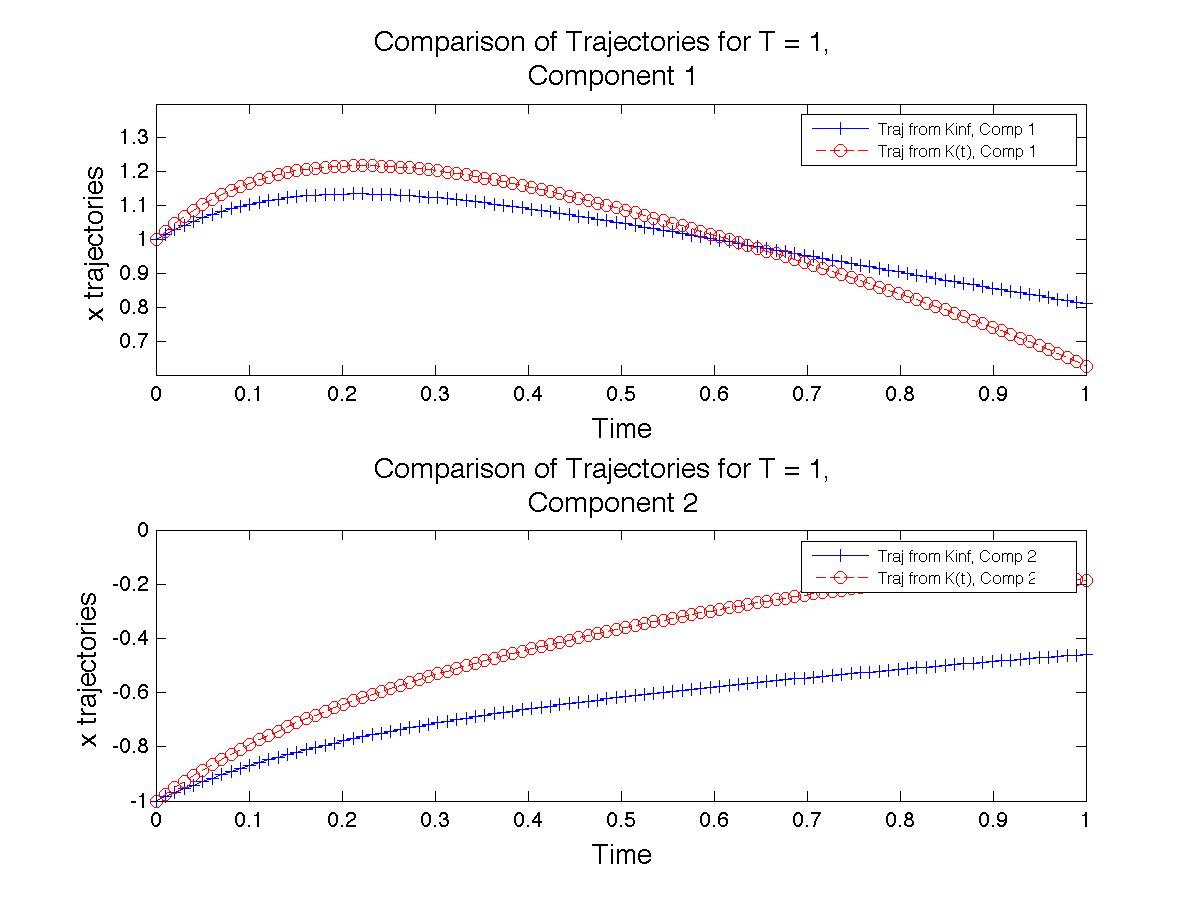
\includegraphics[width=4in]{xCompareT01}
\caption{Comparison of trajectories for $T_1$}
\end{center}
\end{figure}

\begin{figure}[h]
\begin{center}
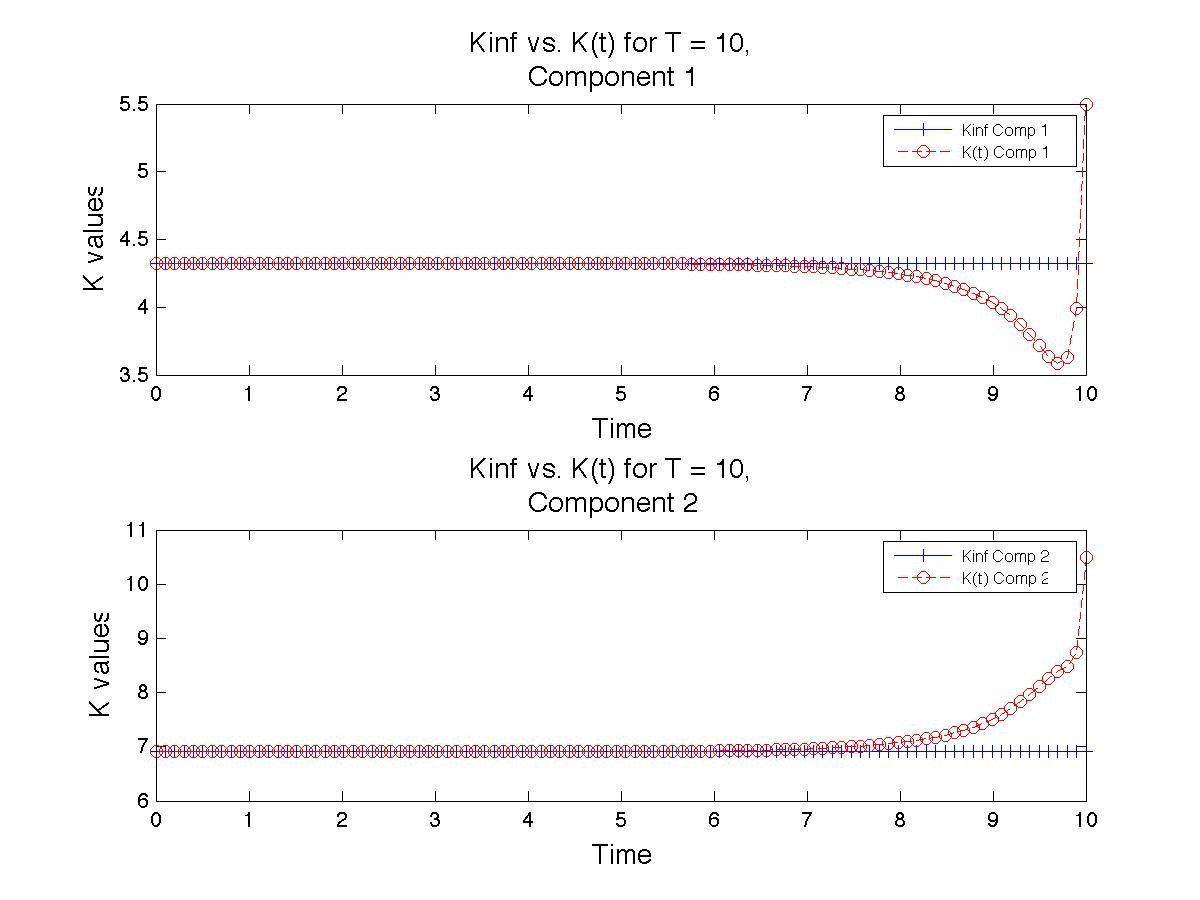
\includegraphics[width=4in]{KCompareT10}
\caption{ Comparison of K's for $T_2$ }
\end{center}
\end{figure}

\begin{figure}[h]
\begin{center}
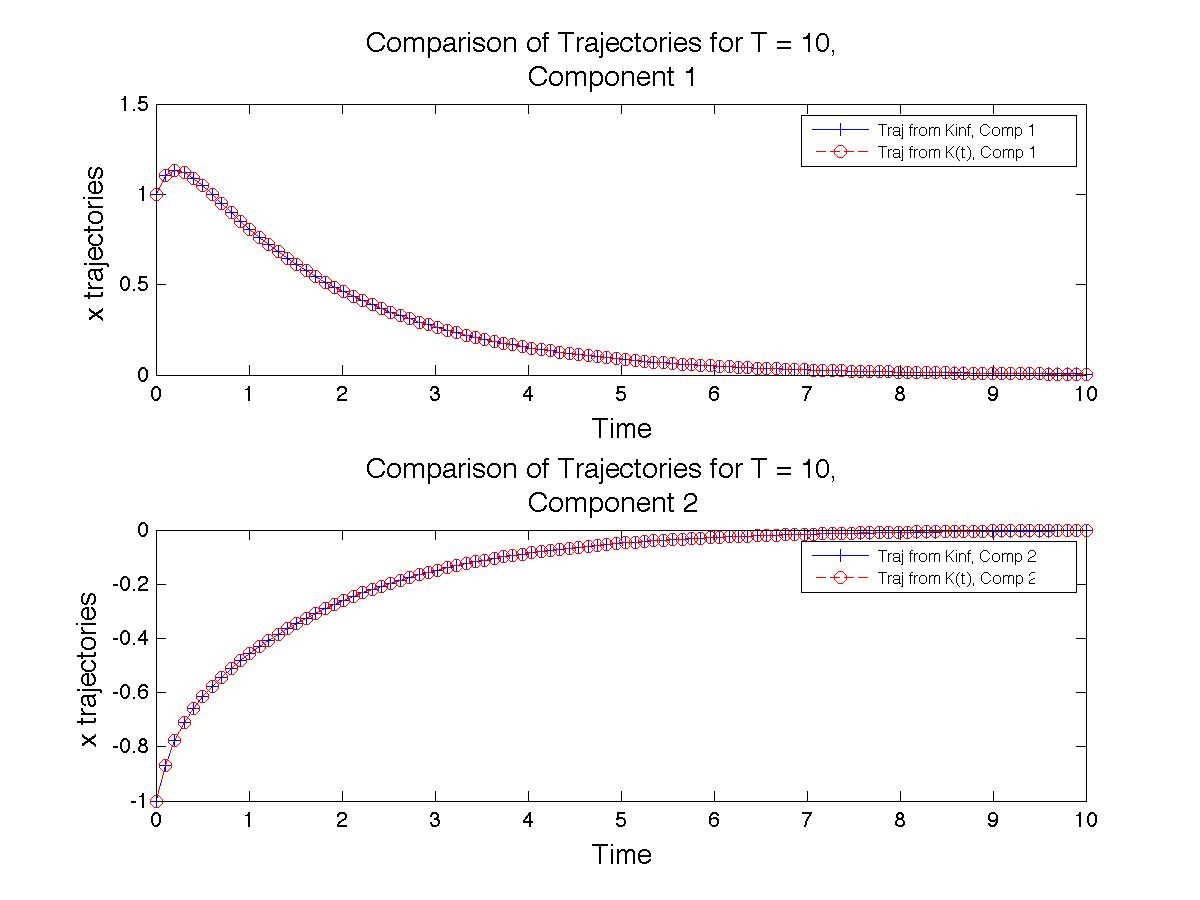
\includegraphics[width=4in]{xCompareT10}
\caption{ Comparison of trajectories for $T_2$ }
\end{center}
\end{figure}



\end{document}